\subsection{D-Latch} % (fold)
\label{sub:D-Latch}
\begin{frame}
    \frametitle{D-Latch}
    \framesubtitle{}
    \begin{figure}[H]
    \begin{center}
            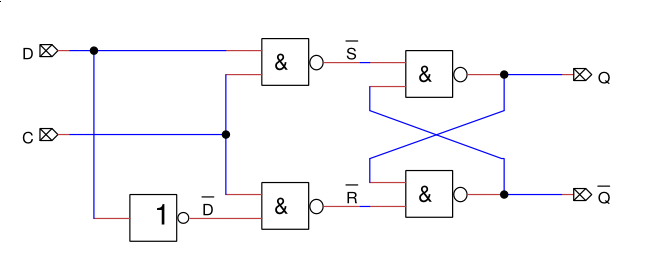
\includegraphics[scale=0.4]{./img/schaltung/d_latch_neu.png}
    \end{center}
    \end{figure}
\end{frame}
\begin{frame}
    \frametitle{Vereinfachung}
    \framesubtitle{}
    \begin{columns}[c]
        \column{0.5\textwidth}
            \begin{figure}[H]
            \begin{center}
                    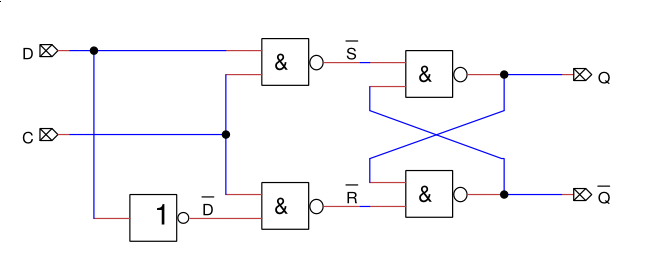
\includegraphics[scale=0.3]{./img/schaltung/d_latch_neu.png}
            \end{center}
            \end{figure}
        \column{0.5\textwidth}
            \begin{figure}[H]
            \begin{center}
                    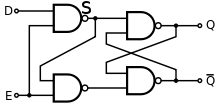
\includegraphics[scale=0.4]{./img/schaltung/D-Latch_2.png}
            \end{center}
            \end{figure}
    \end{columns}
    Betrachte Werte von S: 
            \begin{center}
                \boxed{
                    \begin{tabular}{c|c|c}
                        D & E & S \\
                        \hline
                        0 & 0 & 1 \\
                        0 & 1 & 1 \\
                        1 & 0 & 1 \\
                        1 & 1 & 0 
                    \end{tabular}
                }
            \end{center}
        \begin{block}{}
        \begin{center}
            \begin{itemize}
                \item nur $E=1$ Zustände relevant
                \item S wirkt als invertierer
            \end{itemize}
        \end{center}
        \end{block}
\end{frame}
\begin{frame}
    \frametitle{Funktionsweise}
    \framesubtitle{}
    \begin{columns}[c]
        \column{0.6\textwidth}
            \begin{block}{}
                \begin{itemize}
                    \item Zustand wird geflippt
                    \item Clock (E) muss auf 1 stehen
                \end{itemize}
            \end{block}
        \column{0.4\textwidth}
            \begin{figure}[H]
            \begin{center}
                    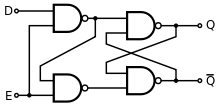
\includegraphics[scale=0.6]{./img/schaltung/D-Latch.png}
            \end{center}
            \end{figure}
            \begin{figure}[H]
            \begin{center}
                    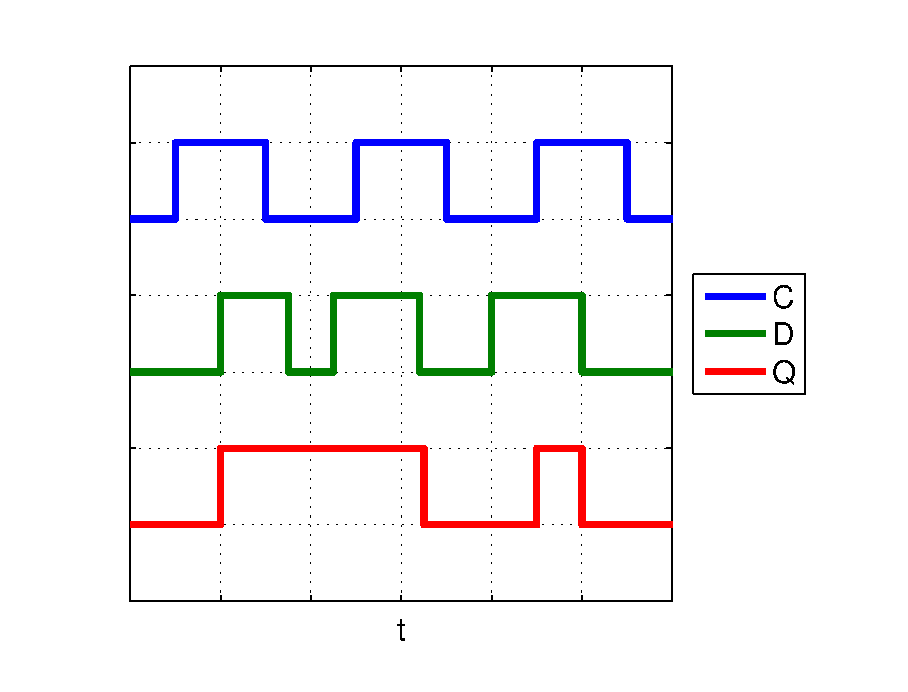
\includegraphics[scale=0.3]{./img/Aufgabe_2_c.eps}
            \end{center}
            \end{figure}
    \end{columns}
\end{frame}
% subsection D-Latch (end)
